\section{Introduction}
  In~\autoref{chap:methods-we}, we gave an overview of common methods to learn
  word embeddings. These methods can leverage different kinds of information
  with diverse model architectures:
  \begin{itemize}
    \item cooccurrence relations of words from a large text corpus to learn
      word embeddings with a single hidden layer neural network
      \citep{collobert2008unified, collobert2011natural,
      mikolov2013distributed};
    \item additional knowledge from external sources of information to capture
      more linguistic information into word
      representations~\citep{yudredze2014improving, kiela2015specializing,
      faruqui2015retrofitting};
    \item or long contextual dependencies of words with deep
      architectures~\citep{peters2018elmo, devlin2019bert}.
  \end{itemize}
  \noindent The objective of these methods is to map each word $w$ of a
  vocabulary $\mathcal{V}$ to a vector representation $\mathbf{v}_w$:

  \begin{equation}
    (w, \mathbf{v}_w)~~\forall w \in \mathcal{V};~\mathbf{v}_w \in \mathbb{R}^d
  \end{equation}

  \noindent where $d$ is the \textit{dimension} of the word embedding,
  \textit{i.e.} the number of values in the vector $\mathbf{v}_w$. Word
  embeddings are usually stored in an \textit{embedding matrix} after they are
  learned by a model and before they are reused into another model. For a
  vocabulary $\mathcal{V}$ of $N_{\mathcal{V}}$ words, the \textit{embedding
  matrix} $\mathbf{M}$ is:

  \begin{equation}
    \label{ch04:eq:embedding-matrix}
    \mathbf{M} \in \mathbb{R}^{N_\mathcal{V} \times d}
  \end{equation}

  \noindent where the $i$-th row is the embedding of the $i$-th word of the
  vocabulary. The size of the embedding matrix is linearly proportional to the
  size of the vocabulary and the number of dimensions of word vectors. As the
  training corpora get bigger and bigger over the years, the size of the
  vocabulary also increases and so is the size of the embedding matrix. As an
  example, for a vocabulary of $N_\mathcal{V} = 2,000,000$ words and vectors of
  $300$ dimensions (common size in the literature) of 32-bits real values, it
  requires $2.4$ gigabytes in memory space to save the embedding matrix ($32$
  bits = $4$ bytes). While this is not a problem when word embeddings are used
  in downtream models on large computing servers, it becomes difficult to use
  them directly on devices with limited memory such as smartphones.\medskip

  Moreover, being able to run models that use word embeddings directly on
  low-resource devices presents other benefits of practical interest. In
  general, smartphones running NLP applications are not powerful enough or do
  not have enough memory to run the models. So they send the data to process to
  large computing servers where the models are able to run. The servers perform
  the calculations and return the results to mobile devices. However, when
  smartphones send to servers user inputs (which can be confidential), servers
  can maliciously store those user inputs for later use instead of only storing
  them to compute the results and returning the results to mobile devices. With
  a model and an embedding matrix small enough to be run locally, the privacy of
  the user is preserved because the user input is not being sent anywhere. If
  the size of word embeddings is reduced, computations can be done locally,
  directly on the embedded device, without needing to send data to the servers.
  The benefits are twofold:
  \begin{enumerate}
    \item Embedded devices can run NLP applications offline, which reduces the
      computing load of servers and can cut down infrastructure costs as less
      servers are required.
    \item Privacy is preserved since no user data is sent to servers.
  \end{enumerate}
  This chapter provides an overview of methods to reduce the size of word
  representations used in downstream models so they can be deployed more easily
  on low-resource devices. It starts with a description of methods which reduce
  the size of the embedding matrix and then presents methods that change the way
  word embeddings are encoded in memory, which also results in the embedding
  matrix taking up less space in memory.

\section{Reducing the size of the embedding matrix}
  As defined in~\autoref{ch04:eq:embedding-matrix}, the embedding matrix is an
  element of $\mathbb{R}^{N_\mathcal{V} \times d}$. To reduce its size, one can
  reduce one (or both) of the dimensions: reducing $d$ will reduce the length of
  each embedding vector (see~\autoref{ch04:subsec:reduce-dimensions}) while
  reducing $N_\mathcal{V}$ means that the number of vectors needed is decreased
  (see~\autoref{ch04:subsec:reduce-words}). Another existing family of methods
  is \textit{distillation}, which transfers the knowledge contained in large
  vectors into smaller word vectors (see~\autoref{ch04:subsec:distillation}).

  \subsection{Reducing the number of vector dimensions}
    \label{ch04:subsec:reduce-dimensions}
    Common word embeddings methods found in the literature usually set a vector
    size of 300~\citep{mikolov2013distributed, pennington2014glove,
    bojanowski2016enriching}. However, not all of the 300 values carry the same
    amount of linguistic information. For example, if a certain dimension has
    almost the same value in all vectors, then this dimension does not bring a
    lot of information to differentiate vectors or to find which ones are the
    most similar together. So this dimension is not really useful for any
    downstream models which use those vectors. The idea of ordering the
    dimensions by their level of encoded information and discarding the less
    important ones is at the root of \textit{Principal Component Analysis}
    (abbreviated \texttt{PCA} thereafter), invented
    by~\citeauthor{pearson1901pca}~\citep{pearson1901pca}. In \texttt{PCA}, the
    level of encoded information in a dimension is computed with its variance.
    The greater the variance, the more information a dimension encodes. But
    \texttt{PCA} does not only compute the variance for each dimension, it also
    finds a transformation that maps the original matrix $\mathbf{M} \in
    \mathbb{R}^{n \times m}$ into a new matrix where the first $p$ dimensions
    ($p < m$) are the ones with the most encoded information. After the
    transformation has been learned and applied to the data matrix, only the
    first $p$ columns are kept. This produces a new data matrix with less
    dimensions where only the most important ones have been kept. To find this
    transformation, \texttt{PCA} starts to compute the covariance matrix
    $\mathbf{C} \in \mathbb{R}^{m \times m}$ of the mean centered matrix of
    $\mathbf{M}$, written as: $\mathbf{M} - \overline{\mathbf{M}}$.

    \begin{equation}
      \mathbf{C} = cov(\mathbf{M} - \overline{\mathbf{M}})
                 = \frac{1}{n - 1} (\mathbf{M} - \overline{\mathbf{M}}){}^\top
                                   (\mathbf{M} - \overline{\mathbf{M}})
    \end{equation}
    Then, eigenvalues and eigenvectors of the covariance matrix $\mathbf{C}$ are
    computed and only the $p$ eigenvectors with the largest eigenvalues are kept
    to form a matrix $\mathbf{P} \in \mathbb{R}^{p \times m}$ (each eigenvector
    has a dimension of $m$). The new data matrix $\mathbf{Q} \in \mathbb{R}^{n
    \times p}$ with a reduced number of dimensions is computed as:

    \begin{equation}
      \mathbf{Q} = \mathbf{M} \mathbf{P}{}^\top
    \end{equation}

    \texttt{PCA} can be applied to any kind of vectors. When applied to word
    embeddings, the number of dimensions of word vectors is decreased. This has
    the consequence of producing smaller vectors which speed up computations in
    downstream models that use them. \texttt{PCA} allows one to reduce the
    number of dimensions while not degrading the performances of word vectors in
    downstream tasks~\citep{lebret2014pca}.\medskip

    While \texttt{PCA} is a good method to reduce the number of dimensions of
    word vectors, it only uses linear projections to find how to transform data
    into a dimension-reduced vector space. It therefore cannot capture
    non-linear dependencies of data present in the original space. To overcome
    this shortcoming, \citeauthor{maaten2008visualizing}
    \citep{maaten2008visualizing} have proposed a new method, called
    \texttt{t-SNE}. It models data of a high-dimensional space with a
    probability distribution between all pairs of vectors. It captures relations
    between close vectors, \textit{i.e.} the local structure of data like
    neighbors, as well as the global structure like clusters. \texttt{t-SNE}
    creates a new vector space for data (with a reduced number of dimensions)
    that follows this learned probability distribution. \texttt{t-SNE} is able
    to reduce the number of dimensions of word vectors. However, it is mainly
    used to visualize data, \textit{i.e.} to project high-dimensional vectors
    into a $2$ or a $3$ dimensional space. When data is projected into a
    $d$-dimensional vector space with $d > 3$, the local structure of data is
    not well preserved because the probability distribution is
    heavy-tailed~\citep{maaten2008visualizing}.\medskip

    \citeauthor{raunak2019effective}~\citep{raunak2019effective} propose another
    method to reduce the number of dimensions of word embeddings. They combine
    \texttt{PCA} with \texttt{PPA}, a \texttt{P}ost \texttt{P}rocessing
    \texttt{A}gorithm applied on learned word embeddings to project the
    embeddings away from the most dominant directions~\citep{mu2018all}.
    \texttt{PPA} applies \texttt{PCA} to the mean centered embedding matrix to
    get the $D$ principal component directions and then remove those $D$
    directions from all the word vectors. \texttt{PPA} does not change the
    number of dimensions of the word vectors but it makes word embeddings more
    discriminative as common dominant directions are removed. Indeed, it has
    been observed that pre-trained word embeddings have usually several common
    mean vectors that are not informative when computing similarity (or
    dissimilarity) between vectors. The algorithm developed by
    \citeauthor{raunak2019effective} starts to apply \texttt{PPA} on a word
    embedding matrix to remove the non informative directions, then applies
    \texttt{PCA} to reduce the number of dimensions and applies again
    \texttt{PPA} on the reduced vectors. Their final embeddings have $50\%$ less
    dimensions compared to the original word vectors and perform better on a
    word semantic similarity task compared to word embeddings that only have
    been processed with a single \texttt{PCA} step (+27\% on average).\medskip

    Reducing the number of dimensions leads to similar or better scores in
    downstream tasks, which can be counter-intuitive because each dimension in
    word embeddings contain information learned during the training step so
    transforming vectors into a lower dimensional space should cause a loss of
    information and worse results. This behavior can be explained by the
    Johnson–Lindenstrauss lemma~\citep{johnson1984extensions}:

    \begin{lemma}[Johnson–Lindenstrauss lemma]
      For any $0 < \epsilon < 1$ and any integer $N_\mathcal{V}$, let $k$ be a
      positive integer such that:
      \begin{equation}
        k \geq \frac{4}{\frac{\epsilon^2}{2} - \frac{\epsilon^3}{3}}
        ~\log(N_\mathcal{V})
      \end{equation}
      Then for any set $X$ of $N_\mathcal{V}$ vectors in $\mathbb{R}^d$, there
      exists a map $f: \mathbb{R}^d \to \mathbb{R}^{k}$ such that for any
      vectors $\mathbf{u}, \mathbf{v} \in X$:
      \begin{equation}
        (1 - \epsilon)\left\lVert \mathbf{u} - \mathbf{v} \right\rVert^2 \leq
        \left\lVert f(\mathbf{u}) - f(\mathbf{v}) \right\rVert^2 \leq
        (1 + \epsilon)\left\lVert \mathbf{u} - \mathbf{v} \right\rVert^2
      \end{equation}
    \end{lemma}

    \noindent This lemma shows the existence of a map function $f$ that can
    project vectors into a lower dimensional space while keeping the distance
    between vectors as close as the distance between the original vectors by at
    most $\epsilon$. The distance between vectors is used to compute their
    similarity, so if the similarity is preserved in the dimensionally reduced
    space then the performances in tasks like document classification or
    sentiment analysis which mainly use vector similarities to perform
    computations are not much affected.

  \subsection{Reducing the number of vectors}
    \label{ch04:subsec:reduce-words}
    As explained at the beginning of this subsection, to reduce the size of the
    embedding matrix $\mathbf{M} \in \mathbb{R}^{N_\mathcal{V} \times d}$, one
    can either reduce the value of $d$ (the number of dimensions in each word
    embedding) or reduce the value of $N_\mathcal{V}$ (the number of vectors in
    the embedding matrix). Usually, the number of vectors is much larger than
    the number of dimensions ($N_\mathcal{V} \gg d$). Indeed, it is common to
    find pre-trained word embeddings with a number of vectors in the order of
    millions while $d$ is typically between 100 and 300. Moreover, in a
    pre-trained word embedding matrix, two similar words are mapped to similar
    vectors (\textit{e.g.} in \texttt{fasttext} pre-trained embeddings, vectors
    of ``road'' and ``highway'' have similar values). Therefore, one can wonder
    if it would be possible to reduce the number of vectors in the embedding
    matrix by associating a common vector to two similar words instead of
    associating two similar (but different) vectors to each one of them. This
    observation is at the root of the method proposed
    by~\citeauthor{shu2018compressing}~\citep{shu2018compressing}. Instead of
    associating each word $w$ to its own embedding vector $\mathbf{v}_w$, it is
    associated with a code $C_w$ composed of $M$ integers between 1 and $K$:

    \begin{equation}
      C_w = (C^1_w,~C^2_w,~\dots,~C^M_w); ~\forall i, ~ C^i_w \in [1, K]
    \end{equation}
    Instead of having one vector for each word, the method creates $M$ codebooks
    (noted as $B_1,~B_2,~\dots,~B_M$), each one composed of $K$ vectors (so $M
    \times K$ vectors in total). The vector $\widetilde{\mathbf{v}}_w$ of a word
    $w$ can be computed by using the integers of its code $C_w$ and summing the
    $C^1_w$-th vector of the first codebook $B_1$, the $C^2_w$-th vector of the
    second codebook $B_2$, etc. This can be written as:

    \begin{equation}
      \widetilde{\mathbf{v}}_w = \sum_{i=1}^M B_i[C^i_w]
    \end{equation}
    where $B_i$ is the $i$-th codebook. This method of summing codebook vectors
    is illustrated in~\autoref{ch04:fig:codebook-embedding}. Vectors in
    codebooks as well as the codes $C_w$ composed of the indexes $C^i_w$ are
    learned with an autoencoder architecture
    (see~\autoref{ch02:subsec:autoencoder} in~\autoref{chap:ml-for-we} for a
    description of autoencoders). The objective of the model is to construct
    compositional vectors $\widetilde{\mathbf{v}}_w$ as close as possible to
    original vectors $\mathbf{v}_w$ for each word $w$ from the vocabulary
    $\mathcal{V}$ of all words in the embedding matrix $\mathbf{M}$. The
    autoencoder model finds the optimal codebook vectors $\hat{B}$ and codes
    $\hat{C}$ by solving the following optimization problem:

    \begin{equation}
      (\hat{B}, \hat{C}) = \argmin_{B, C} \frac{1}{|\mathcal{V}|}
      \sum_{w \in \mathcal{V}}~
      {\left\lVert \widetilde{\mathbf{v}}_w - \mathbf{v}_w \right\rVert}^2
                         = \argmin_{B, C} \frac{1}{|\mathcal{V}|}
      \sum_{w \in \mathcal{V}}~
      {\left\lVert \sum_{i=1}^M B_i[C^i_w] - \mathbf{v}_w \right\rVert}^2
    \end{equation}
    \medskip

    % figure of classic vs. compositional vectors
    \begin{figure}[t]
      \centering
      \begin{subfigure}[t]{0.49\textwidth}
        \centering
        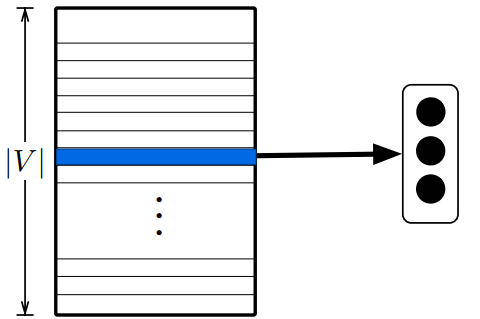
\includegraphics[width=0.75\textwidth]{ch04-codebook-no-compression}
        \caption{Classic embbedings: one vector per word.}
      \end{subfigure} \hfill
      \begin{subfigure}[t]{0.49\textwidth}
        \centering
        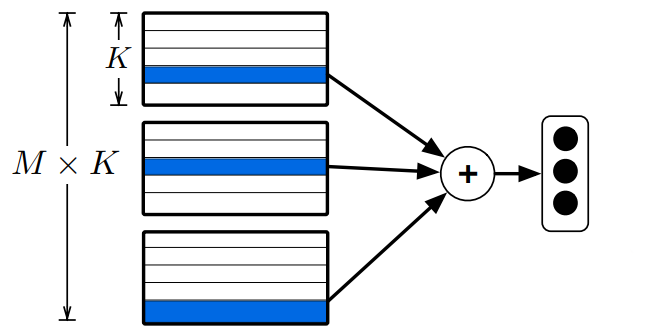
\includegraphics[width=\textwidth]{ch04-codebook-compressed}
        \caption{Codebook embeddings: each word vector is a combination of a
        certain number of base vectors.}
      \end{subfigure}
      \caption[Model used by~\citeauthor{shu2018compressing} to reduce the
      number of word vectors.]{Model used by~\citep{shu2018compressing} to
      reduce the number of word vectors. On the left, the classic word
      embeddings representation where each word is associated to its own vector.
      On the right, there is not a single vector associated to each word but a
      bank of $M \times K$ base vectors. The vector of each word is be computed
      by summing a certain combination of those base vectors.}
      \label{ch04:fig:codebook-embedding}
    \end{figure}

    \noindent Storing base vectors (the codebooks $B_i$) and index codes (the
    $C_w$ codes) instead of all word vectors can drastically reduce the size of
    the embedding matrix. Indeed, with $32$ codebooks of $16$ vectors (so $512$
    base vectors in total), the size of the \texttt{GloVe} embedding matrix can
    be reduced by $98\%$ ($1.23$ megabytes vs. $78$ megabytes) without any
    performances loss in sentiment analysis or machine translation
    tasks~\citep{shu2018compressing}.\medskip

    \citeauthor{chen2018kway}~\citep{chen2018kway} propose a similar idea to
    reduce the number of vectors in the embedding matrix. In the same way, each
    word $w$ is associated to a code $C_w$ of length $M$:
    \begin{equation}
      C_w = (C^1_w,~C^2_w,~\dots,~C^M_w); ~\forall i, ~ C^i_w \in [1, K]
    \end{equation}
    but instead of summing the base vectors corresponding to each $C^i_w$
    like in~\citet{shu2018compressing}, a linear transformation is applied to
    compute the word vectors $\widetilde{\mathbf{v}}_w$:
    \begin{equation}
      \widetilde{\mathbf{v}}_w = H \cdot
                                 \left[ \sum_{i=1}^M B_i[C^i_w]\right]^\top
    \end{equation}
    where $H$ is a $\mathbb{R}^{d \times d}$ matrix and $d$ is the
    dimension of base vectors from the codebooks $B_i$. \citet{chen2018kway}
    also propose another version where base vectors are first passed to a
    LSTM and then combined with a linear transformation:
    \begin{equation}
      \widetilde{\mathbf{v}}_w = H \cdot
                                 \left[ \sum_{i=1}^M h^i_w \right]^\top
    \end{equation}
    where:
    \begin{equation}
      (h^1_w,~h^2_w,~\dots,~h^M_w) = \mathrm{LSTM}(B_1[C^1_w],~B_2[C^2_w],
                                        ~\dots,~B_M[C^M_w] )
    \end{equation}
    \medskip

    \noindent \citeauthor{chen2018kway}~\citep{chen2018kway} learn code
    embeddings in a end-to-end manner: they learn codes and base vectors that
    best work for a given task. This is the main difference compared to the
    method proposed by~\citet{shu2018compressing} which first reduces the size
    of the embeddings and then ``freeze'' code embeddings in the task learning
    step. However, the compressing ratio is the same for both methods (size of
    the embedding matrix is reduced by 98\% without any loss of performances in
    downstream tasks).

  \subsection{Distilling information into smaller embeddings}
    \label{ch04:subsec:distillation}
    Deep architectures like \texttt{ELMo}~\citep{peters2018elmo} or
    \texttt{BERT}~\citep{devlin2019bert} are able to learn word embeddings that
    capture many linguistic information such as meanings, syntax or connotation
    of words thanks to the large number of parameters in their models. However,
    we have seen in~\autoref{ch03:sec:overview-methods}
    of~\autoref{chap:methods-we} that those models are large and it is difficult
    to use them on running environments with limited memory space and small
    computing power. Moreover, large models are often complex and
    over-parametrized to learn as much as possible linguistic information to
    solve multiple tasks, but in practice, not all the parameters are required
    to solve a given task. For example, in a task like sentiment analysis, the
    connotation of a word is more informative than its syntactic properties.  An
    approach to solve this problem is \textit{distillation}. It consists in
    distilling the most useful information required to solve the task
    (\textit{e.g.} the connotation of words in sentiment analysis) into smaller
    models or smaller representations to remove the information not useful for
    the task. Distillation can be applied to:

    \begin{itemize}
      \item the entire model: to reduce the number of parameters required to
        solve the task;
      \item word representations: to reduce the size of representations and
        remove non informative values not required to solve the task. This also
        has the consequence of reducing the size of the downstream model that
        uses smaller representations (see
        \autoref{ch04:fig:distillation-embeddings}).
    \end{itemize}

    \begin{figure}[h]
      \centering
      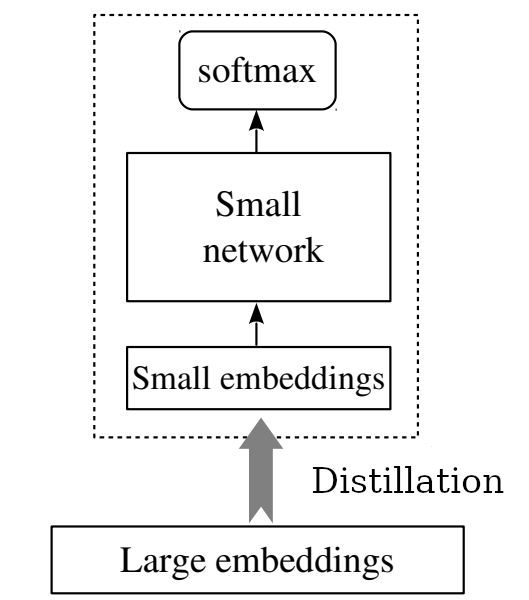
\includegraphics{ch04-distillation-architecture}
      \caption[Distillation of word embeddings.] {Large word embeddings learned
      by large models are tranformed into smaller embeddings before being used
      to solve a downstream task. Linguistic information contained in large word
      embeddings is \textit{distilled} into the smaller ones.}
      \label{ch04:fig:distillation-embeddings}
    \end{figure}

    In the context of this thesis, we are more interested in reducing the size
    of word representations rather than reducing the size of models to solve a
    given task.

    \paragraph{Distillation of trained models.} Given a large model (like a
      neural network) trained on huge datasets, the idea is to train a smaller
      model that replicates the predictions of the large model.
      \citeauthor{hinton2015distilling}~\citep{hinton2015distilling} propose to
      transfer the knowledge learned by the parameters of a large neural network
      to a smaller one by minimizing the distances between the output values of
      the two networks. In this case, output values represent the probability of
      belonging to each possible class, so close output values means that
      the predictions of the small network are similar to the predictions of the large
      network.  \texttt{DistilBERT}~\citep{sanh2019distilbert} is a distilled
      version of the \texttt{BERT} model. The same architecture is kept but half
      of the layers are removed.  \texttt{DistilBERT} is trained to minimize
      three different objective functions: to minimize distances between output
      probabilities of \texttt{DistilBERT} and \texttt{BERT}, to minimize
      prediction errors on annotated examples and to minimize cosine distances
      between internal hidden representations of \texttt{DistilBERT} and
      \texttt{BERT}.

    \paragraph{Distillation of trained word embeddings.} High dimensional word
      vectors trained on a large text corpus with models like \texttt{word2vec}
      or \texttt{GloVe} are transformed into embeddings of smaller dimensions,
      which are then fed into a small model to solve a downstream task (see
      ~\autoref{ch04:fig:distillation-embeddings}). The linguistic knowledge
      captured by large word embeddings is \textit{distilled} into smaller ones.
      \citeauthor{mou2016distilling}~\citep{mou2016distilling} propose to
      distill the knowledge contained in word vectors $\mathbf{v}_w$ of $d=300$
      dimensions into word vectors $\widetilde{\mathbf{v}}_w$ of $d'=50$
      dimensions. The transformation is done with a non-linear neural network
      layer:

      \begin{equation}
        \widetilde{\mathbf{v}}_w = f(\mathbf{W} \mathbf{v}_w{}^\top
                                   + \mathbf{b})
      \end{equation}
      where $\mathbf{W} \in \mathbb{R}^{d' \times d}$, $\mathbf{b} \in
      \mathbb{R}^{d'}$ and $f$ is a non-linear function $f: \mathbb{R}^{d'} \to
      \mathbb{R}^{d'}$. The parameters $\mathbf{W}$, $\mathbf{b}$ and the
      weights of the small downstream neural network which uses the vectors
      $\widetilde{\mathbf{v}}_w$ are learned to minimize prediction errors of
      the output layer on annotated examples. Distilling knowledge into smaller
      word embeddings is different from learning small word embeddings from the
      start.  With a larger number of dimensions, vectors have more freedom to
      capture more linguistic information from a text corpus compared to small
      vectors which have more constraints~\citep{zi2018dimensionality}.
      Additional captured information can then be refined with distillation to
      help solving the downstream task, which is not possible when small vectors
      have been used from the start as they have not captured as much
      information.

    \medskip
    In this section, we have presented methods that reduce the size of the
    embedding matrix by reducing its number of parameters, either by reducing
    the number of dimensions or the number of vectors, or by distilling
    linguistic information into smaller vectors. The next section presents
    methods which use a different approach to reduce the memory size of the
    embedding matrix: by changing the way to encode word vectors.

\section{Encoding word embeddings as integer vectors}
  \label{ch04:sec:integer-vectors}
  To reduce the size of the embedding matrix and use it more easily in
  downstream models on memory-limited devices, we have seen that one can reduce
  its number of dimensions (\autoref{ch04:subsec:reduce-dimensions}) or its
  number of word vectors (\autoref{ch04:subsec:reduce-words}) or distill the
  linguistic information into smaller word vectors
  (\autoref{ch04:subsec:distillation}). In those approaches, the size of the
  embedding matrix can be reduced on average by 98\%. However, this size-reduced
  matrix still uses real-valued vectors. Vector operations done with real values
  are computationally expensive because in modern processors, real-valued
  operations require more processor cycles than operations done with integers.
  Therefore, a size-reduced embedding matrix can be used in a model on a
  memory-limited device but it will be slow to run as those devices often have
  low computing power, especially for real-valued vector operations.\medskip

  Real values (thereafter named \textit{float} or \textit{floating-point}) are
  generally encoded with 32 bits on common machines. If word embeddings are not
  composed of real values (on 32-bits) but of small integer values (on 16-bits),
  the memory size of embeddings is divided by 2 but the computations of vector
  operations are speeded up by a factor greater than 2 because integer
  operations are highly optimized on processors. Therefore, changing the
  representation space of word embeddings and how to encode the information
  captured by those vectors can provide two benefits at the same time: a smaller
  need of memory space and faster vector operations. An alternative
  representation space for word embeddings is the binary space, where each value
  of word vectors is either $0$ or $1$ (a bit) instead of a real value.
  Associating binary vectors to words allows one to speed up computations as
  vector operations can be done with bitwise operators instead of floating-point
  arithmetic, \textit{e.g.} computing the distance between two binary vectors
  only requires a~\verb+XOR+ and
  a~\verb+popcount()+\footnote{\texttt{popcount(n)} returns the number of bits
  set to $1$ in \texttt{n}.} operations (which are both performed with a single
  CPU cycle due to hardware optimizations in modern processors) while it
  requires $\mathcal{O}(n)$ floating-point multiplications and additions for
  $n$-dimensional real-valued vectors to compute their cosine distance. To take
  advantage of fast CPU optimized bitwise operations, the size of binary vectors
  \emph{has to be in adequacy with register sizes} (64, 128 or 256 bits). When
  this criteria is met, computations of vector operations are much
  faster~\citep{norouzi2012fast,subercaze2015metric}. \medskip

  This section details several methods used to produce word embeddings where
  vector values are encoded as integers or as single bits. This has the
  advantage of both speeding up computations of vector operations as well as
  reducing the memory size of the embedding matrix. The methods can be separated
  into two main categories: hashing (described in \autoref{ch04:subsec:hashing})
  and quantization (described in \autoref{ch04:subsec:quantization}).

  \subsection{Hashing of vector representations}
    \label{ch04:subsec:hashing}
    Hashing is a family of methods to transform data from a high-dimensional
    space into a low-dimensional space in order to obtain more compact data such
    that the similarity between two compact items reflect their similarity in
    the original space. One would therefore use the similarity of the compact
    space to find similar items (\textit{e.g.} in a clustering task) because it
    is much faster to compute than the similarity of the original
    high-dimensional space. \citeauthor{charikar2002similarity}
    \citep{charikar2002similarity} propose a \textit{Locality Sensitive Hashing}
    (\texttt{LSH}) method to transform real-valued vectors of $\mathbb{R}^d$
    into a binary space (also called the \textit{Hamming space}) such that the
    similarity between vectors is preserved. They draw a random vector
    $\mathbf{r}$ from a Gaussian distribution over $\mathbb{R}^d$ (\textit{i.e.}
    each dimension of $\mathbf{r}$ is drawn from a Gaussian distribution over
    $\mathbb{R}$) and define a hash function $h_{\mathbf{r}}$ for each vector
    $\mathbf{u} \in \mathbb{R}^d$ as follows:

    \[
      h_{\mathbf{r}} =
      \begin{cases}
            1 & \text{if }\mathbf{r} \cdot \mathbf{u} \geq 0 \\
            0 & \text{if }\mathbf{r} \cdot \mathbf{u} < 0
      \end{cases}
    \]

    \noindent They draw $K$ random vectors from the Gaussian distribution over
    $\mathbb{R}^d$. Each random vector $\mathbf{r}_k$ defines a hash function $
    h_{\mathbf{r}_k}$ and the output of each function are concatenated to
    produce a binary vector of $K$ bits for each vector $\mathbf{u} \in
    \mathbb{R}^d$. Several works have improved locality sensitive hashing either
    by choosing random vectors from a different
    distribution~\citep{datar2004locality} or by using different hashing
    functions~\citep{andoni2006near}.\medskip

    \citeauthor{salakhutdinov2007semantic}~\citep{salakhutdinov2007semantic}
    introduce the concept of \textit{Semantic Hashing} where the objective is to
    find a binary code for each document so semantically similar documents have
    similar codes. Given a query document, its closest neighbors are found by
    only looking at the documents with similar codes instead of looking at all
    the documents. Binary codes are learned with a generative architecture that
    uses Poisson distributions to map Bag-of-Words representations of documents
    to binary codes. Binary codes are then fine-tuned to be able to reconstruct
    the BoW of each document. \citeauthor{weiss2009spectral}
    \citep{weiss2009spectral} propose a method to learn binary codes whose
    Hamming distances approximate the distance of vectors from the original
    vector space $\mathbb{R}^d$. Finding binary codes that exactly preserve this
    distance is a NP-hard problem so the authors relax the problem and remove
    the constraint of having binary codes during training. They learn real-valued
    codes with a spectral decomposition (with eigenvectors and eigenvalues) of
    the similarity matrix $\mathbf{W}$ (where $\mathbf{W}_{i, j}$ is the
    similarity between the $i$-th and the $j$-th vectors from the original
    vector space). Values of eigenvectors are then tranformed to binary features
    with threshold functions, which gives a binary code for each vector.
    \texttt{NASH}~\citep{shen2018NASH} is another architecture used to transform
    real-valued vectors into binary codes for fast similarity searches of
    documents. Their model learns to associate the Bag-of-Words representation
    of a document to a latent vector, which is used to recreate the Bag-of-Words
    representation of this document. During training, latent vectors are
    composed of real values between $0$ and $1$ such that latent vectors follow
    a multivariate Bernoulli distribution. Once the latent vectors have been
    learned, a threshold function is applied to transform them into binary
    codes. Binary latent vectors contain linguistic information because they
    have been trained to reconstruct the Bag-of-Words representations of
    documents.\medskip

    Hashing methods are good approaches to transform real-valued vectors into
    binary codes which are both smaller in memory space and allows one to
    compute vector operations faster. The different models presented in this
    subsection can either use random projections~\citep{charikar2002similarity,
    datar2004locality} or a whole dedicated architecture~\citep{shen2018NASH} to
    find binary codes that preserve the similarities of original vectors. They
    are mainly used to transform the vectors of documents in order to speed up the
    search of similar documents but rarely to transform word embeddings for use
    in downstream tasks because they often fail to fully preserve semantic
    similarities~\citep{Xu2015convolutional}.

  \subsection{Word embeddings quantization}
    \label{ch04:subsec:quantization}
    Common models to learn word embeddings perform operations with real values
    encoded with 32 or 64 bits~\citep{mikolov2013distributed,
    pennington2014glove} but other recent methods are able to learn with
    \textit{half-precision} float \textit{i.e.} real values encoded with 16
    bits~\citep{micikevicius2018mixed, seznec2018study}. Quantization is a
    generic method to reduce the number of bits needed to encode real values.
    For example, if real values have to be encoded with only 4 bits (which gives
    16 possible values because $2^4 = 16$), values need to be rescaled or
    thresholded to be one of the 16 possible values. When the values of vectors
    are encoded with less bits, they require less memory space to be stored.
    This subsection presents different methods to quantize word embeddings and
    therefore reduce their size in memory.\medskip

    \citeauthor{ling2016word}~\citep{ling2016word} shows that word embeddings
    encoded with 64-bits real values can be quantized with values encoded with 8
    bits without any loss of performances in downstream tasks like word semantic
    similarity. The quantization is achieved by rounding the values of vectors.
    To round vector values to $n$-bits precision, values in each vector
    dimension are first scaled so all the vectors values for this dimension lie
    between $[-2^{n-1}, 2^{n-1}]$. The following function is then applied to
    each value $\mathbf{x}_{[i]}$ of each vector $\mathbf{x}$:
    \[
      \text{round}(\mathbf{x}_{[i]}) =
      \begin{cases}
        \lfloor \mathbf{x}_{[i]} \rfloor & \text{if }
          \lfloor \mathbf{x}_{[i]} \rfloor \leq \mathbf{x}_{[i]} \leq
          \lfloor \mathbf{x}_{[i]} \rfloor + \frac{1}{2}\\
        \lfloor \mathbf{x}_{[i]} \rfloor + 1 & \text{if }
          \lfloor \mathbf{x}_{[i]} \rfloor + \frac{1}{2} < \mathbf{x}_{[i]} \leq
          \lfloor \mathbf{x}_{[i]} \rfloor + 1\\
      \end{cases}
    \]
    Each rounded value is then encoded with $n$ bits (since each value is
    between $-2^{n-1}$ and $2^{n-1}$, $n$ bits are enough to encode it). This
    method allows one to choose the value of $n$, the number of bits needed to
    encode each value. This method can also be used to produce binary vectors
    when $n$ is set to 2. However,~\citeauthor{ling2016word} report that the
    performances of binary embeddings (when $n=2$) are worse than the original
    64-bits real-valued vectors whereas the performances stay the same when $n$
    is set to 8.\medskip

    Product Quantization~\citep{jegou2010product} is another method to quantize
    real-valued vectors mainly used for fast similarity searches. Let
    $\mathbf{v}$ be a $d$-dimensional vector ($\mathbf{v} \in \mathbb{R}^d$).
    The vector is split into subvectors $\mathbf{u}_i$ of $m$ dimensions ($d$
    needs to be divisible by $m$).
    \begin{equation}
      \mathbf{v} = (
      \underbrace{\mathbf{v}_1,~\mathbf{v}_2,~\dots,~\mathbf{v}_m
                 }_{\mathbf{u}_1},~
      \underbrace{\mathbf{v}_{m+1},~\dots,~\mathbf{v}_{2m}
                 }_{\mathbf{u}_2},~\dots,~
      \underbrace{\mathbf{v}_{d-m+1},~\dots,~\mathbf{v}_d
                 }_{\mathbf{u}_{d/m}}
      )
    \end{equation}
    The split process is repeated for each vector to quantize. Subvectors are
    quantized separately. For each subvector $\mathbf{u}_i$, a distinct
    $K$-means clustering is done on all the corresponding subvectors of all
    vectors, \textit{i.e.} $K$-means is applied on all the $\mathbf{u}_1$
    subvectors, another $K$-means is applied on all the $\mathbf{u}_2$
    subvectors, etc. The centroids learned by the $i$-th $K$-means algorithm are
    stored in the $i$-th codebook $B_i$. The value of $K$ (the number of
    centroids used in each $K$-means) is selected to be $K = 2^b$ where $b$ is
    the number of bits chosen to encode each subvector. This gives a number of
    possible centroids equal to $2^b$ so each centroid can be assigned to a
    different integer identifier (ID) in $[0, 2^{b}-1]$. After all the $K$-means
    and the codebooks of centroids have been learned (there are $d/m$ $K$-means
    algorithms to perform), each subvector $\mathbf{u}_i$ is assigned to the ID
    of its closest centroid among the corresponding codebook of centroids $B_i$.
    The ID of each subvector are concatenated to obtain a final code for each
    vector $\mathbf{v}$. \citet{jegou2010product} use the product quantization
    (PQ) method for fast similarity retrieval among the description vectors of
    images. Real-valued vectors are transformed to 64-bit binary codes and
    provide a better recall@1 (\textit{i.e.} the number of times the closest
    vector in the original space is the closest vector in the binary space) than
    other methods like spectral hashing~\citep{weiss2009spectral}.\medskip

    An original use of product quantization is made in
    \texttt{fasttext.zip}~\citep{joulin2016fasttext} to transform word embedding
    into compact codes for a more efficient memory text classification
    architecture. The same method as in product quantization is used to get a
    binary code for each word, which are then used in a downstream
    classification model composed of a single hidden layer neural network.
    However, computations performed inside the downstream model are not done
    with binary codes. To compute operations between two binary codes, the codes
    are first \textit{de-concatenated} to get the ID of each centroid used to
    quantize each subvector $\mathbf{u}_i$. Vector operations are then performed
    with the respective centroid vector of each subvector $\mathbf{u}_i$. The
    objective of \texttt{fasttext.zip} is to reduce the size of the model for a
    classification task, not to speed up computations between vectors which is
    why operations are not done with binary codes but with real-valued vectors
    (the centroid vectors). With further optimization tricks like keeping only
    the most discriminative words of the vocabulary for the task,
    \texttt{fasttext.zip} can reduce the size of the classification model by a
    factor of 1000 with a loss of performances around $0.8\%$ for a document
    classification task.\medskip

    In product quantization, vectors are split sequentially: subvectors
    $\mathbf{u}_1$ use the dimensions from $1$ to $m$, subvectors $\mathbf{u}_2$
    use the dimensions from $m+1$ to $2m$, etc. However, the quantization
    distortion (the difference between quantized vectors and original ones) can
    be reduced by reorganizing the dimensions as the distances between vectors
    and their assigned centroid is dependent on the values of vectors and thus
    on the range of values in each dimension. \citeauthor{ge2013optimized}
    \citep{ge2013optimized} propose an \textit{Optimized Product Quantization}
    (OPQ) method in which they learn the way to reorganize the vector space to
    split subvectors in addition to learning the centroids. Re-ordering the
    dimensions of vectors $\mathbf{v} \in \mathbb{R}^d$ can be represented by an
    orthogonal matrix $\mathbf{R} \in \mathbb{R}^{d \times d}$. The authors
    learn both the matrix $\mathbf{R}$ and the codebooks of centroids $B_i$ that
    minimize the quantization error:

    \begin{equation}
      \min_{\mathbf{R}, B_1, \dots, B^{d/m}} \sum_{\mathbf{v}}
        \left\lVert \mathbf{v} -
                    c(\mathbf{u}_1,~\dots,~\mathbf{u}_{d/m}) \right\rVert^2
    \end{equation}
    where $\mathbf{u}_i$ is the $i$-th subvector of the rotated vector
    $\mathbf{R} \mathbf{v}$, $c$ is the concatenation of the centroid vectors
    assigned to each $\mathbf{u}_i$, and $\mathbf{R}$ is an orthogonal matrix
    such that $\mathbf{R}{}^\top \mathbf{R} = \mathbf{R} \mathbf{R}{}^\top = I$.
    This objective function is minimized by alternatively optimizing two steps:
    in the first step, the matrix $\mathbf{R}$ is freezed and only the codebooks
    are learned with the classic product quantization method; in the second
    step, the codebooks and the centroids are freezed and only $\mathbf{R}$ is
    learned, which is equivalent to find the rotation of vectors that minimize
    the distance between their subvectors and their closest respective centroid vector
    (which are freezed). Compared to product quantization, OPQ greatly increases
    the recall rate with 64-bit binary codes (0.71 against 0.41 for PQ on
    recall@100) on MNIST images.\medskip

    Quantization methods are mainly used for fast retrieval. Indeed, most of the
    methods presented in this subsection use quantized vectors for fast
    similarity searches~\citep{jegou2010product, ge2013optimized, ling2016word}.
    The compact representations are not learned to be used in downstream models
    to solve NLP tasks. Even in \texttt{fasttext.zip} which uses product
    quantization to reduce the size of a document classification model,
    computations are not performed with quantized vectors but with the
    real-valued cluster vectors used to learn the quantized vectors. Since
    quantized vectors are not learned to preserve the linguistic properties of
    original word vectors but rather to preserve the similarity between vectors,
    some linguistic information is lost during quantization. For example, it has
    been shown that real-valued word embeddings are able to capture word
    analogies~\citep{mikolov2013distributed} which indicates that vector
    dimensions can represent specific linguistic relations. But in binary
    vectors, one bit (or a group of bits) cannot be associated to a specific
    linguistic feature. \citeauthor{faruqui2015sparse} \citep{faruqui2015sparse}
    propose a method to quantize word embeddings so dimensions in binary vectors
    are more interpretable. Binary vectors are generated by learning a linear
    transformation that maps pre-trained word embeddings into a larger
    dimensional space (usually with 10 times more dimensions) where the values
    of vectors are positive and $90\%$ of them are set to $0$ (we call them
    \textit{sparse} vectors). Binary vectors are then obtained by setting all
    the non-zero values to 1. \citeauthor{faruqui2015sparse} show that sparse
    binary vectors have bits symbolizing specific linguistic features. For
    example, binary vectors associated to words of animals have bits in common
    that other vectors do not have. While sparse binary vectors are useful to
    find interpretable features, the size reduction ratio is not as high as in
    other quantization methods. Sparse binary vectors have a length of 3,000
    bits while product quantization or optimized product quantization learn
    binary codes which have a length between 64 and 256 bits. Therefore, the
    approach of \citeauthor{faruqui2015sparse} is interesting from a linguistic
    point of view because of the interpretability of dimensions in vectors, but
    is limited from a memory-efficient storage point of view.

\section{Conclusion}
  Word embeddings are real-valued vectors learned to capture linguistic
  properties of words. When the number of vector dimensions is high (most common
  methods use vectors of 300 dimensions) or when the number of words to
  represent is important (vocabulary can contain millions of words), the
  embedding matrix which contain the embeddings of all the words of the
  vocabulary becomes large and prevents downstream model which use it to be run
  on memory-limited devices such as smartphones. In this chapter, we have
  presented methods to reduce the size of the embedding matrix as well as
  methods to learn more compact word embeddings with alternative encodings of
  values which also have the benefit of speeding up vector computations. Methods
  to reduce the size the embedding matrix can be divided into two main
  categories:

  \begin{itemize}
    \item by reducing the dimensions of the embedding matrix;
    \item by changing how the values of word embeddings are stored in memory.
  \end{itemize}
  To reduce the dimensions of the embedding matrix, one can either reduce the
  number of dimensions of word embeddings or reduce the number of vectors in the
  matrix. \texttt{PCA} \citep{pearson1901pca} or \texttt{t-SNE}
  \citep{maaten2008visualizing} are common methods to reduce the number of
  dimensions of vectors by finding a transformation that keeps only the $k$ most
  informative directions of vectors. Another method to reduce the number of
  dimensions is to \textit{distill} the knowledge captured by large word
  embeddings into smaller word embeddings with either a neural network
  architecture~\citep{mou2016distilling} or a reduced version of an existing
  model~\citep{sanh2019distilbert}. To reduce the number of vectors stored in
  the embedding matrix, a solution is to consider that each word embedding can
  be written as a combination of a certain amount of base vectors. Instead of
  storing one vector for each word, only the base vectors and the list of base
  vectors to combine for each word are stored, which reduces the number of
  vectors to store. \citet{shu2018compressing} propose to sum base vectors
  while~\citet{chen2018kway} propose to use linear combinations of base vectors.
  In both methods, using base vectors (typically 512 base vectors) reduces the
  size of the embedding matrix by $98\%$ without any loss of performances of
  word embeddings in downstream tasks.\medskip

  Another type of approaches to reduce the memory size of word embeddings is to
  change how their values are encoded. In common word embeddings models, vectors
  use real values encoded with 32 bits. \citet{ling2016word} propose to round
  values so only the first 8 bits are kept. This has the consequence of reducing
  the size of the embedding matrix by 4 without any loss of performances in
  downstream tasks. Product quantization \citep{jegou2010product} is another
  method that transforms real-valued word vectors into binary codes by applying
  $K$-means algorithms on separate subvectors and concatenating the ID of the
  closest centroid of each subvector to form a binary code for each word. This
  method has been applied to word embeddings to reduce the size of a document
  classification model~\citep{joulin2016fasttext}. Binary word embeddings use
  less memory space and have the advantage of speeding up vector computations as
  operations on binary vectors are much faster than vector operations performed
  with real-valued vectors~\citep{norouzi2012fast, subercaze2015metric}.\medskip

  We have seen in the previous chapter that \textit{good} word embeddings encode
  a lot of linguistic information so downstream models which use them have more
  knowledge about the language and can perform better in NLP tasks. But they
  require large models and representations that cannot be used in memory-limited
  environments.  Methods presented in this chapter allows one to reduce the size
  of word representations in memory by trying to minimize the loss of
  information during the size reduction step. The compact word embeddings are
  mainly used for retrieval and fast similarity searches, not for use in
  downstream models to solve NLP tasks.  The challenge is therefore to find
  methods that can transform large word embeddings which contain a lot of
  linguistic information into compact representations which preserve this
  linguistic information and are small enough to be used on those limited
  environments. This challenge is one of the main topic of this thesis
  and~\autoref{chap:nlb} presents a contribution that answers it with a new
  method to transform word embeddings into compact binary codes that can be used
  in downstream NLP tasks.
